\section{Load Swings and Energy Storage}

One consequence of GPUs being synchronized is that their workloads and therefore power profiles are also synchronized. This has been a problem in supercomputers for decades but is now becoming widely understood as a challenge during AI factory deployments. During a typical LLM workload there are intervals of intense matrix computation followed by intervals exchanging data. Unmitigated, this leads to rapid swings from idle at approximately 30\% of rack power to 100\% power utilization. This becomes a problem not only for the rack power distribution, but with large enough cluster sizes, it is an issue at the datacenter level and even the power grid.

\begin{figure}[h]
\centering
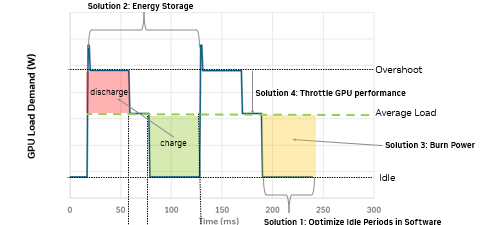
\includegraphics[width=0.8\textwidth]{figures/figure_p5_i1.png}
\caption{Energy storage to flatten the load demand}
\label{fig:load-flatten}
\end{figure}

To deal with these load swings there are multiple approaches that can be taken as seen in Figure~\ref{fig:load-flatten}: Energy storage to flatten the load demand.

\begin{description}
\item[Solution 1 -- Optimize Idle Periods in Software] If these idle periods can be minimized in software this is the ideal solution since it reduces datacenter power requirements.

\item[Solution 2 -- Energy storage] This is an energy efficient method to deal with these load swings is to use energy storage. Energy storage allows charging during the idle periods and discharging during the peaks to low pass filter the rack current demand. This energy storage can come in multiple forms, electrolytic capacitors, supercapacitors, batteries, etc.

\item[Solution 3 -- Burn Power] This is done in the Nvidia GPU via the Power Smoothing feature. This allows for burning power after a delay so that power only burned after the limit of the energy storage has been reached. This is not ideal on it's own, but in conjunction with energy storage can provide a backstop for longer idle periods than the local energy storage can maintain.

\item[Solution 4 -- Throttle GPU performance to reduce peaks] These software controls are available in the Nvidia GPUs, but this is not ideal because it can reduce performance with some workloads.
\end{description}

All 4 solutions can be used together to provide a comprehensive load swing mitigation strategy. Ideally the energy storage is used to cover a majority of the load swing durations while burning power and throttling performance only act as a backstop in corner cases.

\begin{figure}[h]
\centering
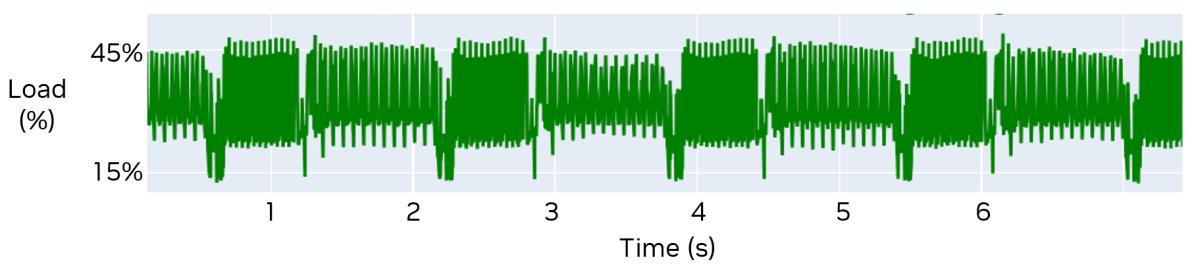
\includegraphics[width=0.8\textwidth]{figures/figure_p6_i1.jpeg}
\caption{GPU Load Swings during an LLM workload}
\label{fig:gpu-load-swing}
\end{figure}

Looking across the GPU workload in Figure~\ref{fig:gpu-load-swing} are events at multiple timescales. Looking at the overall system, there are grid level fluctuation requirements and the GPU load demand requirements. Energy storage needs to fill the gap between these two conflicting requirements; the grid needs a stable predictable load, and the GPU needs a very dynamic source.

GPU overshoots known as the Electrical Design Point (EDPp) and peak power consumption and typical workload idle periods are in the range of up to 100ms, checkpointing can take 1 to 5 seconds, and then the workload ramp up and ramp down needs to occur over several minutes. In addition, depending on the use case, energy storage might be required as transition power to ensure that the load remains operational even during the transfer to a backup power source after a loss of primary power.

\begin{figure}[h]
\centering
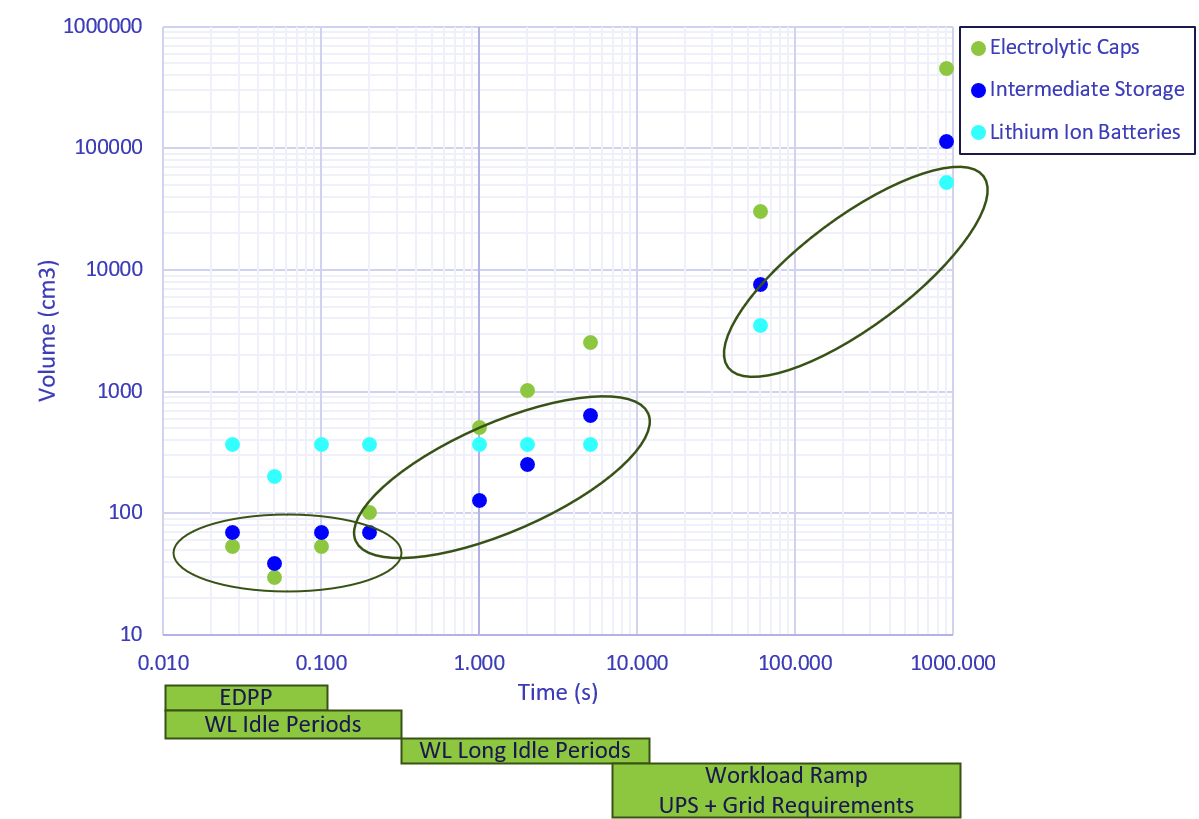
\includegraphics[width=0.8\textwidth]{figures/figure_p7_i1.png}
\caption{Volume of energy storage by technology vs. time duration}
\label{fig:storage-volume}
\end{figure}

Figure~\ref{fig:storage-volume} above shows volume of different energy storage solutions vs. time. Volumetrically electrolytic capacitors are a good solution for anything below 100 ms. There is a mix of solutions that are more optimized for the period between 100 ms and 10 seconds and then beyond this timescale batteries are the better volumetric solution. Mitigating the load swings as close as possible to the GPU is desired to keep slew rates on the datacenter manageable as well as to reduce the RMS current increases. A square wave with a 50\% duty cycle and a 50\% peak over the average then going back to idle will result in a 25\% increase in RMS losses. Equipment in the datacenter needs to be sized to handle the peak current of the rack as well as the increase in RMS losses so reducing these peaks as close as possible to the GPU is valuable for reducing overall datacenter equipment costs and impacts.
